\chapter{Lyrics-to-Audio Alignment}
\label{sec:alignment}

\section{Automatic Alignment}

Automatic lyrics-to-audio alignment is a problem that might seem similar to the problem of automatic speech recognition. However, some characteristics of singing voice are very different from the ones of speech, which prevents the usage of speech recognizer for performing the alignment.

Firstly, acoustic characteristics, such as pitch and loudness, tend to fluctuate much more in singing than in speech. Secondly, sounds in singing, especially vowels, tend to be prolonged or shortened, which results in larger variation of sound duration compared to speech \citep{Kruspe.2018}. The background music is the third difference between singing and speech. As the spectrum of singing voices gets affected by accompaniment sounds, it makes the process of lyrics-to-audio alignment more difficult \citep{Fujihara.2012}. For this reason, some studies prefer working with unaccompanied singing rather than with polyphonic music.

Some minor difficulties of recognizing or aligning singing voice also include lyrics-specific vocabulary, which differs from vocabulary used in spoken language \citep{Kruspe.2018}, and incomplete song texts, especially due to omitting interjections such as \textit{oh} or \textit{yeah} \citep{Fujihara.2012}.

As was briefly mentioned above, there are studies aiming at singing voice recognition e.g. \cite{Kruspe.2018} and \cite{Sasou.2005}, as well as the ones concentrating on lyrics-to-audio alignment. In this thesis, only works on alignment of singing voices to songs texts will be reviewed. There is also some research done on unaccompanied singing \citep{Loscos.1999, Sasou.2005, Gong.2015}. However, the task of lyrics-to-audio alignment in polyphonic music is more suitable for the future Android application, so studies on unaccompanied singing are left out in this evaluation.

The granularity of lyrics-to-audio synchronization can be different --- possible fragments of lyrics include phoneme \citep{Mauch.2012}, syllable \citep{Iskandar.2006}, word, phrase \citep{Fujihara.2006, Dzhambazov.2016}, line \citep{Wang.2008, Wong.2007, Mesaros.2008}, paragraph \citep{Lee.2008} and section \citep{Wang.2008}, which, depending on the interpretation, can correspond to paragraph-level alignment. Among the works that are analyzed in this section, synchronization on line level is chosen for the greatest number of studies. This granularity of synchronization is also the best option for the Android application that is being developed.

As could be expected, most authors choose songs in English to evaluate their approach. There are, however, singular studies that concentrate on other languages, such as Japanese \citep{Fujihara.2006, Fujihara.2008}, Cantonese \citep{Wong.2007} and Turkish \citep{Dzhambazov.2016}. To the best of my knowledge, no systems have been analyzed on songs in German.

It is unclear how many songs should be included in the test set to provide reliable results, but, except for one work where the system was tested on three songs only \citep{Iskandar.2006}, studies typically include from ten to twenty songs in their test set.

Metrics used to evaluate how successful a system performs the alignment task often differ from one study to another, which makes it difficult to compare results between various studies, especially if the granularity of synchronization is also different. Evaluation metrics include average displacement error \citep{Wang.2008, Lee.2008, Mesaros.2008}, average word error rate \citep{Iskandar.2006} and average accuracy \citep{Fujihara.2006, Fujihara.2008, Mauch.2012, Dzhambazov.2016}, with average accuracy being the most popular metric. Among systems evaluated with the accuracy metric, the best one achieves accuracy of 0.88 on a phoneme level \citep{Mauch.2012}. If one chooses average displacement error as an evaluation metric, the smallest error\footnote{A mean error of 7.34 and 9.03 seconds has been achieved in \cite{Kruspe.2018}, but it is hard to compare this result to other works due to their different granularity.} would be 0.58 seconds on a line level \citep{Wang.2008}. Both systems are tested on English songs.

Unfortunately, even though the two systems show rather impressive result, they are not publicly available. Moreover, the accuracy of synchronisation is crucial for the app, as it ensures interactive learning, and even an error of  half-a-minute would make a difference. Apart from that, if some of the methods used in the systems appear to be language-specific, the systems would also not be applicable for songs in German. In addition, not too many songs are included in the app initially. Due to these reasons, manual lyrics-to-audio alignment was preferred over automatic alignment.

\section{Manual Alignment}

There are several programs that support the process of manual lyrics-to-audio alignment.

\subsection{GNMIDI}

This program is only available for Microsoft Windows users, and offers a possibility to manually align half of the lyrics in its free version\footnote{Demo version of GNMIDI 3.17 was tested.}. The user pastes the text of the song as a whole and aligns the lines of the lyrics to the audio by pressing the \textit{Enter} key when a line is sung. In this way, a file of LRC format is created, where every line of the lyrics is assigned the time when it is sung (see Figure \ref{fig:lrcFormat}\footnote{Example taken from \url{https://en.wikipedia.org/wiki/LRC_(file_format)}}). In files of this format, the time is usually written as \textbf{[mm:ss.xx]}, where \textbf{mm} stands for minutes, \textbf{ss} --- for seconds, and \textbf{xx} --- for hundredths of seconds. 

\begin{figure}[H]
    \begin{verbatim} 
        [00:12.00]Line 1 lyrics
        [00:17.20]Line 2 lyrics
        [00:21.10]Line 3 lyrics
        ...
        [mm:ss.xx]last lyrics line  \end{verbatim}
    \caption{LRC Format}
    \label{fig:lrcFormat}
\end{figure}

When the user exports the resulting file from GNMIDI, however, no hundredths of seconds are saved in the file. The karaoke demonstration in the program (see Figure \ref{fig:karaokeDemo}) also relies on times without hundredths of seconds. 

\begin{figure}[H]
    \centering
    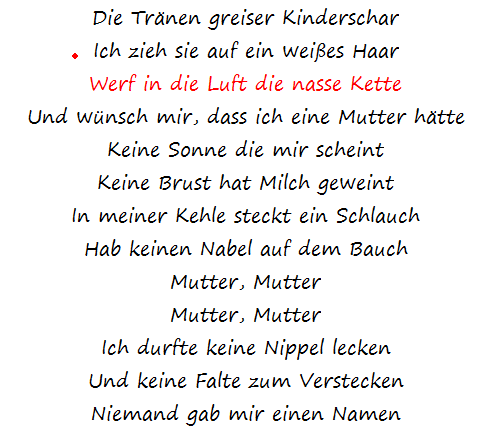
\includegraphics{images/gnmidiScreenshot.png}
    \caption{GNMIDI Karaoke Demonstration (song \textit{Mutter} by Rammstein)}
    \label{fig:karaokeDemo}
\end{figure}

Apart from that, GNMIDI does not support UTF-8 format, which is important for lyrics in German.

\subsection{SYLT Editor}

SYLT Editor is a free software, and versions both for Microsoft Windows and Linux are available\footnote{SYLT Editor 1.1 was tested for this section.}. In contrast to GNMIDI, the program supports UTF-8 encoding. However, loading LRC-format file with lyrics has failed, so the song text had to be entered line by line. After the user assigned times to lines of the lyrics by pressing the \textit{Space} button when a line is sung, the text should be able to be exported to a file of LRC format. Unfortunately, exporting a file, as well as importing a file, was not possible due to an occurring error.

\subsection{Megalobiz: LRC Maker \& Generator Online}

LRC Maker \& Generator Online is a website\footnote{\url{https://www.megalobiz.com/lrc/maker}} where one can align lyrics to audio of the song after loading an MP3-file and pasting in the text of the song. When a line is sung, the user must click on this line for it to be assigned the time. The user can also check if he/she aligned the lines in a right way by playing the song again --- the lines of the lyrics will be highlighted according to assigned times. To save the file in LRC format, the user should press the button \textit{Save}, which results in a UTF-8 encoded file on his/her computer.

To sum up, LRC Maker \& Generator Online is the best choice for manual lyrics-to-audio aligning, as it saves the hundredths of seconds in time tags, in contrast to GNMIDI, and is able to export the resulting file, unlike SYLT Editor. Moreover, the website is completely free to use. The website was used for tagging song texts used in the Android app.